\documentclass[preprint]{aastex62}

% \usepackage{minted}
\usepackage{listings}
\usepackage{courier}
\usepackage{cleveref}
\usepackage{float}

\definecolor{bcolor}{RGB}{0, 51, 153}
\definecolor{gcolor}{RGB}{51, 153, 51}

\shorttitle{photon counting \& detectors}
\shortauthors{j. birky}

\begin{document}

\title{\sc Lab 1: Photon Counting \& Detectors}
\author{Jessica Birky, Julian Beaz-Gonzalez, Russell Van-Linge}

\correspondingauthor{Jessica Birky (A13002163)}
\email{jbirky@ucsd.edu}

\begin{abstract}
In this lab, we examine the statistics of photon counting, and the noise properties of a charged couple device (CCD) from 2048x2048 pixel optical images taken on the Nickel 1 meter direct imaging camera. In particular we characterize the effect of several types of noise: first the inherent noise of photon counting by comparing to the Poisson distribution, second the read noise associated with the dark current in the detector, and lastly we comment the effect of different systematics such as instrument defects or dark current due to temperature variations. In total we collect XX frames integrated at varying exposure times ranging from 0 to 768 seconds. Comparing the slope between mean and variance of each bias-subtracted, combined frame of each exposure, we determine the gain of the detector to be XX ADU/s. Normalizing our frames (dividing the counts by exposure time) we find that as we add more exposures, the mean of the mean (MOM) detector counts per second converges to XX ADU/s and the standard deviation of the mean (SDOM) decreases to XX ADU/s with more frames added.

\end{abstract}
\bigskip

\section{Introduction} 
In order to understand the. Advancements in technology in the 20th century has now made it possible to observe electromagnetic radiation from the scales of $10^{-12}-10^3$m (as short as gamma rays to as long as radio waves). Understanding how detectors work, the statistics of light collection, as well as the limitations of the instrument and sources of contaminations are a fundamental first steps before performing any scientific analysis of light with an instrument.

CCDs, the photoelectric effect

Types of noise we want to quantify

% ==================================
\section{Observations}
Observations are taken on the Nickel 1 meter telescope, located  (Table \ref{table:log})

\begin{table}[H]
\centering
\begin{tabular}{|c|c|c|c|c|}
    \hline
    Start File \# & End File \# & \# Frames & Type  & Exposure Time (sec) \\
    \hline
    \hline
    401 & 404 & 5 & Bias & 0  \\
    420 & 421 & 2 & Flat & 3 \\
    422 & 425 & 4 & Flat & 6 \\
    426 & 428 & 3 & Flat & 12 \\
    429 & 431 & 3 & Flat & 24 \\
    432 & 434 & 3 & Flat & 48 \\
    435 & 437 & 3 & Flat & 96 \\
    438 & 439 & 2 & Flat & 192 \\
    440 & --  & 1 & Flat & 384 \\
    441 & --  & 1 & Flat & 768 \\
    \hline
\end{tabular}
\caption{Observation log, recording the files associated with each exposure time. Files $405-418$ were removed due to inconsistent count numbers.} \label{table:log}
\end{table}


% ==================================
\section{Data Reduction \& Methods}
\subsection{Theoretical Distribution of Light}
Before we can characterize our observations, it is important to first determine what we expect our data will look like. That is, we are measuring the number of photons hitting a detector over a fixed amount of time, what do we predict will be the number of photons that will hit each pixel in that tme interval? Let's assume that on average $\mu$ photons will hit a pixel over fixed time interval $t$. Now consider dividing that time interval into $n$ increments: the probability that a $n$ photons arrive to the detector is approximately Binomial. Now in the limit that $n\rightarrow\infty$, we arrive at the Poisson distribution:
\begin{equation}
P(x;\mu) = \frac{\mu^x}{x!}e^{-\mu}
\end{equation}
which we interpret as the probability that x photons will arrive to a detector pixel in time interval $t$, given that $\mu$ photons arrive in that interval on average. The expected mean and variation for this distribution being $\langle x \rangle = \mu$ and $\langle \sigma^2 \rangle = \mu$. 

In practice, the Poisson distribution is unstable to compute for large values of x because the term $x!$ becomes too large for the memory of the computer to handle. In order to try to reduce the memory load for large values of x, we approximate the $x!$ term using the Sterling approximation:
\begin{equation}
n! \sim \sqrt{2\pi n}\left(\frac{n}{e} \right)^n
\end{equation}
the code for the Poisson distribution is implemented in lines $7-9$ of Appendix \ref{code:stats}.

However when the conditions for the Poisson distribution are not met very well (average number of successes is much smaller than the probable value ($\mu << n$), and the number of counts are low), the Gaussian distribution may instead be a good approximation:
\begin{equation}
P(x; \mu, \sigma) = \frac{1}{\sqrt{2\pi}} e^{-\frac{(x-\mu)^2}{2\sigma^2}}
\end{equation}
where the input parameters are the mean and standard deviation of the data ($\mu$ and $\sigma$). The code for the Gaussian distribution is implemented in lines $11-13$ of Appendix \ref{code:stats}. 

\subsection{Data Reduction} \label{sec:reduction}
For each exposure observed, the data output from the Nickel instrument is stored in a fits file, which contains the two-dimensional array of detector counts at each pixel, as well as other relevant variables about the detection (such as the detector temperature, time of observation, exposure time, etc.). The first step of reduction consists of combining the bias frames, and our procedure for combining frames (lines $19-26$, \ref{code:data}) is to take the median count value at each pixel. Second, for each exposure, we read the individual files from a directory, subtract the combined bias, then combine those into a single frame (lines $9-11$, \ref{code:reduction}).

As discussed in further the results (\ref{subsec:diagnostic})

\subsection{Types of Detector Noise} \label{subsec:noise}
How to calculate the readnoise, other noise, error propagation

\begin{equation}
\sigma_{ADU}^2 = \frac{ge}{C} \left(ADU - ADU_0 \right) + \sigma_0^2
\end{equation}
Thus the gain (ge/C) is the linear slope between the mean and variance of the ADU counts for each bias-subtracted, combined exposure frame. To numerically determine the gain from our data we fit a second-order polynomial to our mean vs. variance plot (lines $1-7$, \ref{code:gain}), and the gain is then the first order term (coefficient of x).

% ==================================
\section{Data Analysis \& Modeling}

\subsection{Diagnostic Plots: Combined Images \& Histograms} \label{subsec:diagnostic}
Figure \ref{fig:bias} shows the combined bias frames, and the figures in \ref{fig:flats1} and \ref{fig:flats2} show the bias-subtracted, combined histograms and images for each of the eight different exposure times (3, 6, 12, 24, 48, 96, 192, 384, and 768 seconds), using the procedures described in \ref{sec:reduction}. Lines $25-33$ of \ref{code:plots} plots the histogram, and lines $72-75$ plot the image.

The left side of each panel shows the histogram of the number of detector counts in analog to digital units (ADU), normalized such that the sum of all of the bins is one (plotted in black). The solid blue vertical line marks the mean of the data, and the dashed blue line marks the median, indicating which distrubtions are symmetric or skewed. For all histograms however, the mean and median are very close, meaning the distributions are quite symmetric. The two shades of green mark $\pm1$ and $\pm2$ standard deviations above and below the mean. Finally, the distribution in red shows the expected Poisson distribution, as a function of the mean of the data ($\bar{x}$), with a one standard deviation range also shaded in red (where the expected standard deviation for the Poisson is $\sigma=\sqrt{\bar{x}}$). The distribution in cyan shows the Gausian fit using the mean and standard deviation of the data ($\bar{x}, s$). The Poisson and Gaussian distributions are scaled to the data by first normalizing to one, then multiplying by the max frequency of the data (lines $50-51$ and $58-59$, \ref{code:plots}).

The right side of each panel shows the 2D images. In order to visualize the detector counts per pixel, we must map the number of counts to an RGB color value, which we use the {\tt matplotlib} `gray' colormap for. To emphasize the features in the data, we choose the min an max values of the colormap to be the 10th and 90th percentile counts of the data.

\begin{figure}[H]
\plotone{plots/exposure0.png}
\caption{Combined bias frames.} \label{fig:bias}
\end{figure}

\subsection{Mean of the Mean \& Standard Deviation of the Mean}
For each of our bias-subtracted frames, we divide the arrays by their exposure times to put them on the same scale of counts per second, and we take the means (giving us a 1x27 array of the average values for 27 frames). Next we compute the mean of the mean (MOM) and standard deviation of the mean (SDOM) in a for loop (lines $1-37$, \ref{code:mom_sdom}): the first MOM/SDOM are the mean and standard deviation of the first frame taken, the second is the MOM/SDOM for the first two frames, and so on. The resulting plot (Figure \ref{fig:mom_sdom}) shows how the standard deviation decreases with larger N (more number of observations) and the mean stays roughly constant because the normalized distributions are centered around roughly the same peak.

\begin{figure}[H]
\begin{center}
\includegraphics[width=.48\linewidth]{plots/mom_sdom.png}
\caption{Mean of the mean and standard deviation of the mean vs. number of frames taken. \textit{Credit: Russell}} \label{fig:mom_sdom}
\end{center}
\end{figure}

\subsection{Quatifying Detector Noise}
Figure \ref{fig:mean_var} is the mean vs. variance plot for each bias-subtracted, combined exposure. As described in \ref{subsec:noise} we fit a second-order polynomial using {\tt numpy} to the point on the plot. The fit is mostly described by the first-order gain term which is XX, with a very small second-order correction of XX.

\begin{figure}[H]
\begin{center}
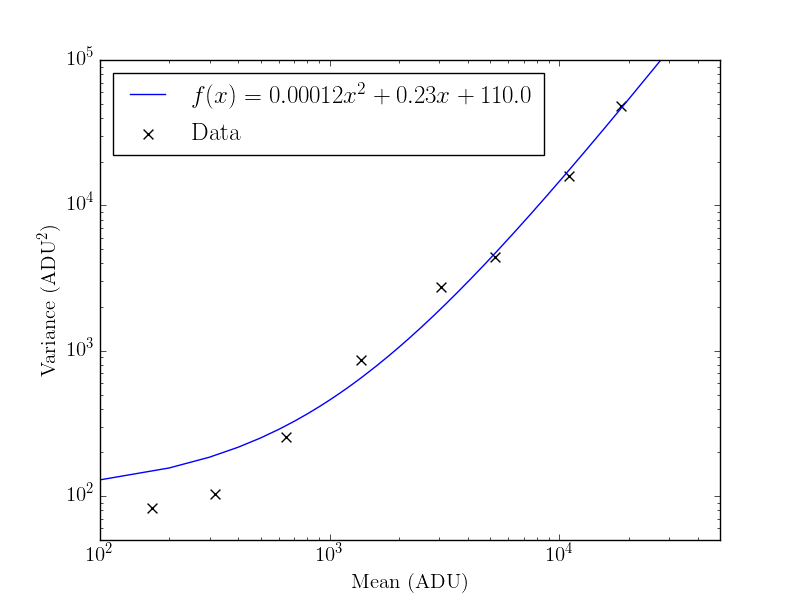
\includegraphics[width=.48\linewidth]{plots/mean_vs_variance.png}
\caption{Mean vs. variance for all bias-subtracted exposures, fitted to a second-order polynomial.} \label{fig:mean_var}
\end{center}
\end{figure}

% ==================================
\section{Discussion}
\subsection{Poisson \& Gaussian Comparisons} \label{subsec:dist_comparisons}


\subsection{Sources of Noise \& Systematic Effects}
Looking at the full 2048x2048 images we found that the detector count distribution was close to a Poisson distribution for low exposure times, but for larger exposure times it increasingly diverges with a much larger standard deviations than expected. We also saw that low exposure times (3, 6, and 12 sec) have a single peak in the distribution around the mean, however at 48 sec the distribution becomes bimodal, and for high exposure times (96, 192, 384, and 768 sec) the distribution develops three separate peaks. 

Variations in the quantum efficiency of each pixel, and vignetting of the image.
Dust particles on the lens scatter and absorb light unevenly at different points on the detector.

Checked for systematics due to temperature variation that could maybe be responsible for dark current: found temperature to vary only within 4C (Figure \ref{fig:temp}). Checked for systematic differences in different datasets. 

\begin{figure}[H]
\begin{center}
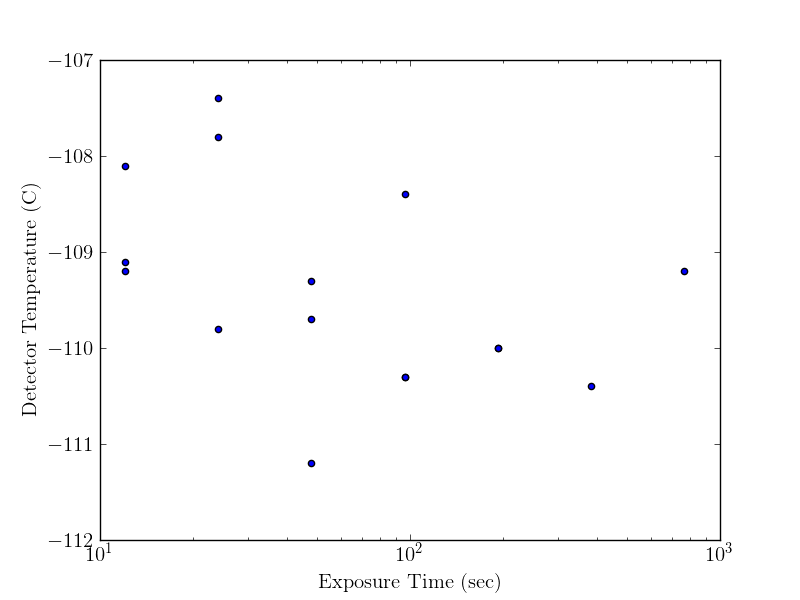
\includegraphics[width=.48\linewidth]{plots/exposure_temp.png}
\caption{Temperature of the CCD detector for different exposure frames does not vary more than about 4C.} \label{fig:temp}
\end{center}
\end{figure}

% ==================================
\section{Conclusion}


% ==================================
\section{Author Contributions}

This project was done in collaboration with Julian Beas-Gonzalez and Russell Van-Linge (Group E), using data collected by Group B. Russell wrote code for fitting Poisson and Gaussian distribtions and computing MOM/SDOM, Julian wrote code for histograms and computing MOM/SDOM, and I wrote code for combining frames/bias subtracting images, plotting histograms/images and slicing images (except for a few snippets for making histograms and reading fits files from the class notes). We met several times outside of class to compare results, fix issues, and combine our code together, which can be found on github: \href{https://github.com/jbirky/photonCounting}{https://github.com/jbirky/photonCounting}.

\begin{figure}[H]
\plotone{plots/exposure3.png}
\plotone{plots/exposure6.png}
\plotone{plots/exposure12.png}
\plotone{plots/exposure48.png}
\caption{Combined, bias-subtracted, flat frame histograms and images for varying exposure times (0, 3, 6, and 12 sec). \label{fig:flats1}}
\end{figure}
\begin{figure}[H]
\plotone{plots/exposure96.png}
\plotone{plots/exposure192.png}
\plotone{plots/exposure384.png}
\plotone{plots/exposure768.png}
\caption{Combined, bias-subtracted, flat frame histograms and images for varying exposure times (96, 192, 384, and 768 sec). \label{fig:flats2}}
\end{figure}

% ==================================
\newpage
\section{Appendix}

\lstset{language=Python,
        basicstyle=\footnotesize\ttfamily,
        keywordstyle=\color{blue},
        numbers=left,
        numberstyle=\ttfamily,
        stringstyle=\color{red},
        commentstyle=\color{gcolor},
        morecomment=[l][\color{gray}]{\#}
}

\subsection{Statistical Code} \label{code:stats}
\small
\hrule
\begin{lstlisting}
def mean(array):
    return np.sum(array)/len(array)

def stdev(array):
    return np.sqrt(sum((array - mean(array))**2)/(len(array) - 1))

def poisson_approx(data, mean):
    pdist = np.array(np.exp((data*np.log(mean))-(data*np.log(data))+data-mean))
    return pdist

def gaussian(data,mean,sigma):
    gdist = np.array((1/(sigma*(2*math.pi)**(.5)))*np.exp(-.5*((data-mean)/sigma)**2)) 
    return gdist
\end{lstlisting}
\hrule \vspace{7pt}

\subsection{Data Processing code} \label{code:data} 
\hrule
\begin{lstlisting}
def readData(folder):
    """
    Read all frames from a given directory into one matrix.
    input:  directory to folder containing frames
    output: array3d (dimension: xpixel x ypixel x # frames)
            array2D (dimension: 1D flattened img x # frames)
    """
    
    files = os.listdir(folder)

    array3D, array2D = [], []
    for ff in files:
        arr = fits.getdata(folder + ff)
        array3D.append(arr)
        array2D.append(arr.flatten())
    
    return np.array(array3D)

def combineFrame(data_array):
    """
    Combine image frames and return 1D array.
    input:  data array (dimension: # 1D detector counts x # frames)
    output: 1D combined array of detector counts (ADU)
    """
    
    return np.median(data_array, axis=0)
\end{lstlisting}
\hrule \vspace{7pt}

\subsection{Histogram/Image code} \label{code:plots} 
\hrule
\begin{lstlisting}
def plotAll(array2D, **kwargs):
    
    arr = array2D.flatten()
    
    avg = mean(arr)
    std = stdev(arr)
    med = np.median(arr)
    Npix = len(arr)    
    
    sigma = kwargs.get('sigma', 2)
    low = int(np.round((avg-sigma*std)))
    high = int(np.round((avg+sigma*std)))
    rng = kwargs.get('rng', [low, high])
    exp = kwargs.get('exp')
    if 'nbins' in kwargs:
        nbins = kwargs.get('nbins')
        bin_size = (rng[1]-rng[0])/nbins
    else:
        bin_size = kwargs.get('bin_size', 1)
    
    fig, (ax1, ax2) = plt.subplots(1,2, figsize=[18,6])
    
    # Histogram
    #===========
    hr = np.arange(rng[0], rng[1]+1, bin_size)
    hist = []
    for i in range(len(hr)):
        try:
            counts = len(np.where((arr >= hr[i]) & (arr < hr[i+1]))[0])
        except:
            counts = 0
        hist.append(counts)
    ax1.step(hr, hist, color='k')

    #mean and median lines
    ax1.axvline(avg, color='b', label=r'$\bar{x}=%s$'%(np.round(avg,2)))
    
    #sigma levels
    if kwargs.get('show_level', True) == True:
        for i in np.arange(1,sigma+1):
            if i == 1:
                ax1.axvspan(avg-i*std, avg+i*std, facecolor='g', alpha=0.05, \
                    label=r'$s=\pm %s$'%(np.round(std,2)))
            else:
                ax1.axvspan(avg-i*std, avg+i*std, facecolor='g', alpha=0.05)
                
                
    #poisson distribution
    xarray = np.arange(rng[0]-10, rng[1]+10, 1)
    pdist = poisson_approx(xarray, avg)
    pdist = max(hist)/max(pdist)*pdist
    ax1.plot(xarray, pdist, color='r', label=r'$P_{Poisson}(\bar{x})$')
    std_expected = math.sqrt(avg)
    ax1.axvspan(avg - std_expected, avg + std_expected, facecolor='r', alpha=0.05, \
                label=r'$\sigma=\pm %s$'%(np.round(std_expected,2)))
    
    #gaussian distribution
    gdist = gaussian(xarray, avg, std)
    gdist = max(hist)/max(gdist)*gdist
    ax1.plot(xarray, gdist, color='c', label=r'$P_{Gaussian}(\bar{x}, s)$')
    
    ax1.legend(loc='upper left')
    ax1.set_xlabel('Counts (ADU)')
    ax1.set_ylabel('Frequency')
    
    if 'exp' in kwargs:
        ax1.set_title('Combined Histogram (Exposure Time: %s sec)'%(exp))
    ax1.set_xlim(rng)
    
    # Image
    #===========
    hrng = kwargs.get('hrng', [np.percentile(arr, 10), np.percentile(arr, 90)])
    pl = ax2.imshow(array2D, origin='lower', interpolation='nearest', \
         cmap='gray', vmin=hrng[0], vmax=hrng[1])
    fig.colorbar(pl, ax=ax2, fraction=0.046, \
                 pad=0.04).set_label('Detector Value (ADU)')
    
    ax2.set_xlabel('pixels(x)')
    ax2.set_ylabel('pixels(y)')
    ax2.set_title('Combined Image')
    
    if 'save_dir' in kwargs:
        save_dir = kwargs.get('save_dir')
        plt.savefig(save_dir + 'exposure%s.png'%(exp))
    plt.show()
\end{lstlisting}
\hrule \vspace{7pt}

\subsection{Data Reduction} \label{code:reduction} 
\hrule
\begin{lstlisting}
files = natsorted(os.listdir('data/'))[1:]
exp_times = np.array([int(f.split('exp')[1]) for f in files])

#combined frames, and combined frames in counts per second
counts, counts_ps = [], []
for exp in exp_times:
    
    #Read frames, subtract combined bias, combine frames
    array3D = readData('data/exp%s/'%(exp))
    bias_sub_3D = [(frame - bias_2D) for frame in array3D]
    array2D = combineFrame(bias_sub_3D)
    
    array2D_cps = array2D/exp
    
    #cut out safe part of image
    cut = Cutout2D(array2D, window[0], window[1]).data
    cut_cps = Cutout2D(array2D_cps, window[0], window[1]).data
    
    counts.append(cut.flatten())
    counts_ps.append(cut_cps.flatten())
    
    #Plot histogram and image & save to .png
    plotAll(cut, sigma=3, exp=exp, show_level=True, save_dir='writeup/plots/')
\end{lstlisting}
\hrule \vspace{7pt}

\subsection{Gain Calculation} \label{code:gain} 
\hrule
\begin{lstlisting}
xbar = np.mean(counts, axis=1)
s = np.std(counts, axis=1)

#fit polynomial
x_arr = np.arange(0, 10**5, 10**2)
fit = np.polyfit(xbar, s**2, 2)
y_arr = np.polyval(fit, x_arr)
\end{lstlisting}
\hrule \vspace{7pt}

\subsection{MOM and SDOM Calculation} \label{code:mom_sdom} 
\hrule
\begin{lstlisting}
files = np.array(natsorted(os.listdir()))
data = []

# Go through each frame, take the median, subtract bias, and divide 
# by exposure time
for i in files:

    # loading in the data
    frame_data = fits.getdata(i)
    frame_exp = fits.open(i)
    exp_time = frame_exp[0].header['EXPTIME']
    # Subtracting the bias
    data_subbed = frame_data - bias_2D
    data_median_ps = np.median(data_subbed,axis=0)/exp_time
    # Median of each frame divided by exposure time for that frame
    data.append(data_median_ps)
   
data = np.array(data)

# Setting up arrays 
mom = []
std = []
num_frame = np.arange(2,len(data)+1)

# Calculates MOM and SDOM 
i = 2
while i < len(data)+1:
    frames = data[:i]
    mean = np.mean(frames) 
    stand = np.std(frames)
    mom.append(mean)
    std.append(stand)
    i = i + 1

plt.scatter(num_frame,mom,marker='x',color='black',label='MOM')
plt.scatter(num_frame,std,marker='v',color='gray',label='SDOM')
plt.show()
\end{lstlisting}
\hrule \vspace{7pt}

% \lstinputlisting[language=Matlab]{./Code/calc_error.m}

% \begin{thebibliography}{}
% \bibitem[Astropy Collaboration et al.(2013)]{2013A&A...558A..33A} Astropy Collaboration, Robitaille, T.~P., Tollerud, E.~J., et al.\ 2013, \aap, 558, A33 
% \end{thebibliography}


\end{document}

